\documentclass{beamer}
\usepackage[utf8]{inputenc}
\usepackage{graphicx}
\usepackage{color}
\usepackage{hyperref}
\hypersetup{
    colorlinks=true,
    linkcolor=blue,
    filecolor=magenta,      
    urlcolor=cyan,
}
%\usetheme{Hannover}
\newcommand{\hilight}[1]{\textbf{\textcolor{structure.fg!85}{#1}}}
\setbeamertemplate{footline}[frame number]

\author[Sowmya Vajjala]{Sowmya Vajjala}

\title[SfSNLP]{NLP without Annotated Dataset}
\subtitle{NLP: An Introduction}
%: \\ on using insights from language acquisition, cognitive science and psychology research

\date{8 January 2021}

\institute{Seminar f\"ur Sprachwissenschaft, University of T\"ubingen, Germany}
%%%%%%%%%%%%%%%%%%%%%%%%%%%

\begin{document}

\begin{frame}\titlepage
\end{frame}

\begin{frame}
\frametitle{Outline}
\begin{enumerate}
    \item \textbf{What is NLP?}
    \item The many faces of NLP
    \item What makes NLP Challenging?
    \item Some common NLP Tasks: An overview
     \item The levels of language processing: some examples    
     \item Approaches to NLP
\end{enumerate}
\end{frame}

\begin{frame}
\frametitle{}
\bigskip
\Large What is NLP?
 \\
\tiny note: images without source attribution are taken from our book: practicalnlp.ai 
\end{frame}


\begin{frame}
\frametitle{What is NLP?}
\begin{itemize}
\item NLP is a sub-field of Artificial intelligence that is concerned with analyzing, modeling and understanding human language using computational methods. \pause \item The eventual goal is to make computers understand (and generate) human languages, and make them communicate with humans like humans
\pause \item Because of its role in the process of human-computer interaction, NLP has a wide range of technological applications
\pause \item It is also becoming popular as a research method in a broad range of disciplines in social sciences. 
\end{itemize}
\end{frame}


\begin{frame}
\frametitle{Inter-disciplinary by nature}
NLP is very inter-disciplinary. Draws from research in Computer Science, Linguistics, Mathematics, Statistics, Psychology etc.,
\end{frame}

\begin{frame}
\frametitle{Computational Linguistics vs NLP}
The terms are used synonymously. However, generally, NLP is typically used by people involved in engineering and technology development, and CL is typically used by traditionally linguistics groups who adapted computational methods.
\end{frame}

\begin{frame}
\frametitle{History of NLP}
\begin{enumerate}
\item Foundational ideas: 40s and 50s. WWII and Beyond.
\item Main NLP problem of that time (and even now): Machine Translation
\item First few decades: Work focused on the development of speech recognition systems, logic based language understanding systems, creating elaborate grammars to teach human language to computers, rule based systems, and automatic language generation.
\item Late 90s on: Advent of statistical methods and machine learning
\item 2010s: Deep learning
\item Last few years: more into interpretable models, discussion about ethical issues, introspection about the field etc. 
\end{enumerate}
\end{frame}

\begin{frame}
\frametitle{Where is NLP useful in real world?}
\begin{itemize}
    \item general purpose applications: search, email, voice based assistants on phones etc.
    \item domain specific applications: e-commerce, legal, finance, health care etc. 
    \item educational technology: language teaching, learning, assessment tools 
    \item language revitalization software
    \item disaster management tools 
\end{itemize}
... 
\end{frame}

\begin{frame}
\frametitle{}
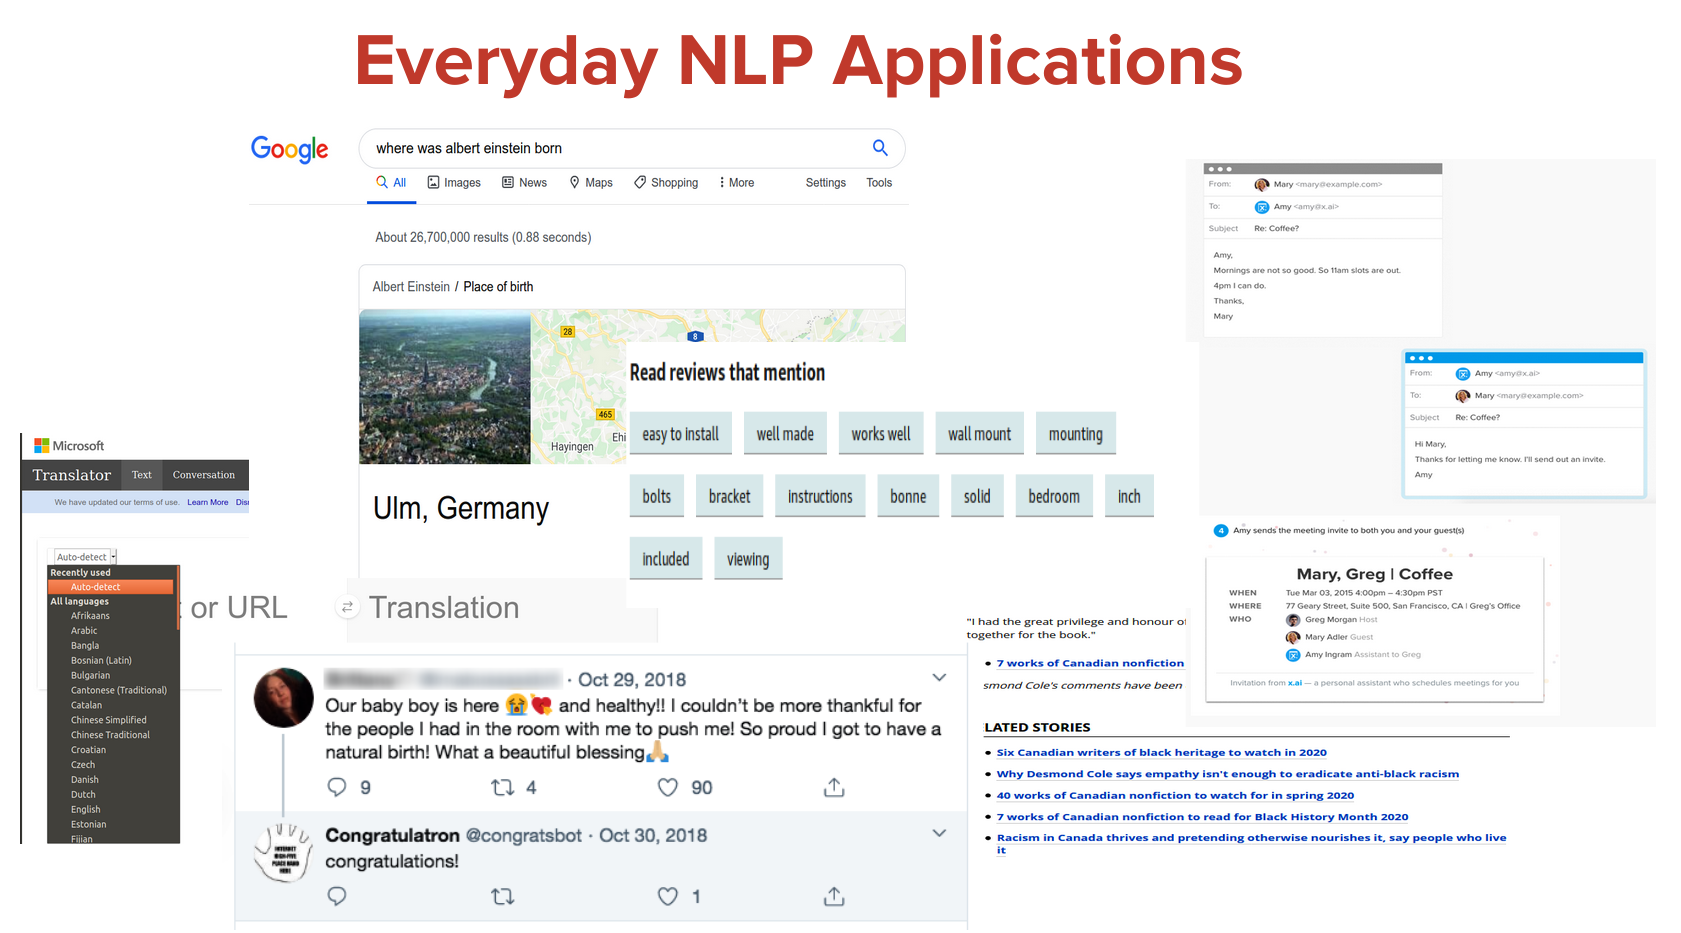
\includegraphics[width=\textwidth]{figures/everydaynlp.png}
\end{frame}

\begin{frame}
\frametitle{Where is NLP used in real-world?}
\begin{enumerate}
\item Apple Siri, Google assistant and other such software 
\item Google Translate and the likes
\item Search Engines
\item Question Answering (e.g., IBM Watson)
\item Sentiment analysis of product reviews on Amazon, for example
\item Spam classification in Gmail, Yahoomail etc
\item Information extraction from text (e.g., identifying calendar entries automatically in gmail)
\item Spelling/Grammar check tools, language learning apps such as DuoLingo etc.
\end{enumerate}
\end{frame}

\begin{frame}
\frametitle{Where is NLP used elsewhere?}
\begin{enumerate}
\item NLP is used as a method to answer research questions in many disciplines.
\item NLP sometimes plays a major role in discipline specific challenges, going beyond being just a research method.
\item In Google Scholar, I saw mentions of NLP methods in journals as diverse as Asian studies \& History to Clinical Oncology.
\end{enumerate}
\end{frame}

\begin{frame}
\frametitle{Outline}
\begin{enumerate}
    \item What is NLP?
    \item \textbf{The many faces of NLP}
    \item What makes NLP Challenging?
    \item Some common NLP Tasks: An overview
    \item The levels of language processing: some examples
    \item Approaches to NLP
\end{enumerate}
\end{frame}

\begin{frame}
\frametitle{}
\bigskip
\Large The Many Faces of NLP
\end{frame}


\begin{frame}
\frametitle{The many faces of NLP}
Three broad groups: 
\begin{enumerate}
\item NLPers: NLP researchers in academia and industry
\item Other researchers who use NLP methods in their research
\item Industry professionals developing NLP based applications
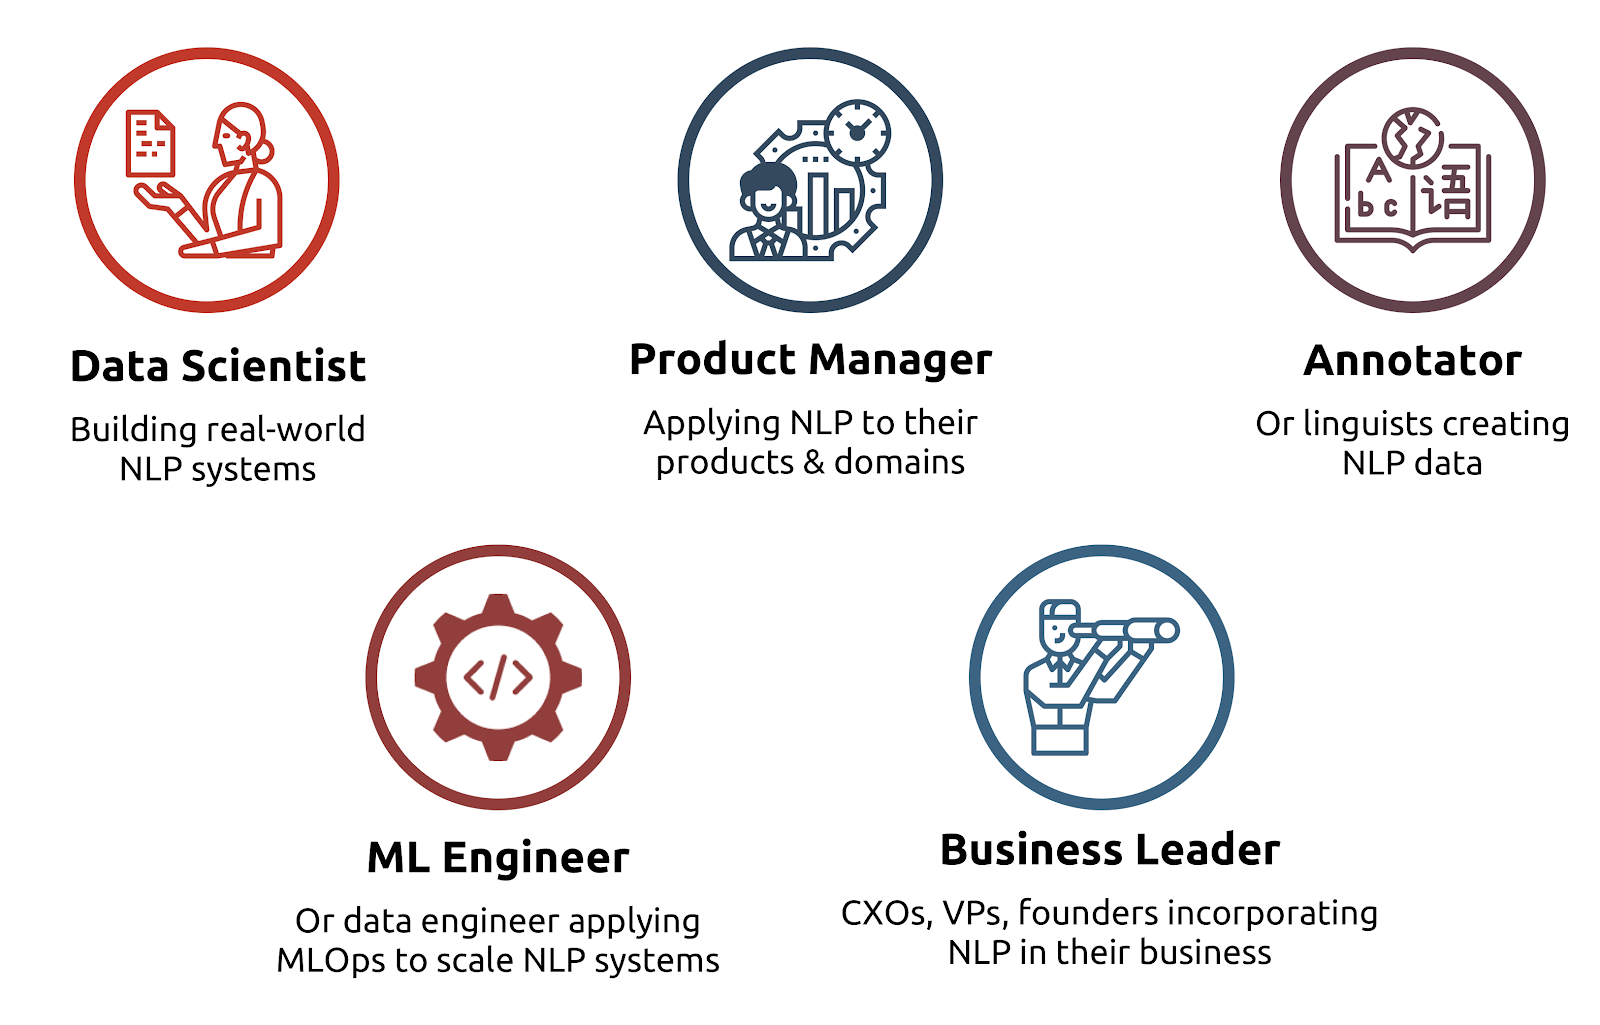
\includegraphics[width=\textwidth]{figures/nlpindustry.png}
\end{enumerate}
\end{frame}

\begin{frame}
\frametitle{NLP research - an overview}
A snapshot of contemporary NLP research topics
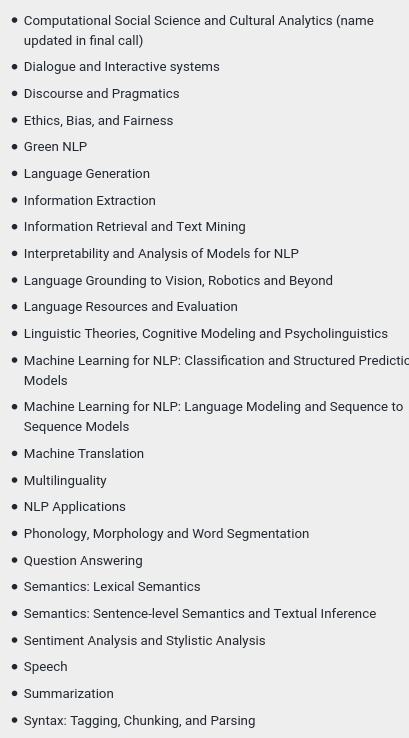
\includegraphics[width=0.3\textwidth]{figures/naacl2021areadesc.png}
(source: \url{https://2021.naacl.org/calls/papers/})
\end{frame}

\begin{frame}
\frametitle{Trends in NLP Research}
How can one quickly showcase contemporary NLP research to others?
$\Rightarrow$ Some paper titles from best paper awards over the past 5 years may give a picture.
\\ source: \url{https://aclweb.org/aclwiki/Best_paper_awards} and 2020 conference websites.
(everything is open access!)
\end{frame}

\begin{frame}
\frametitle{Contemporary NLP Research - 1}
A lot of research focuses on what can perhaps be called core NLP tasks and applications:  
\begin{itemize}
    \item \href{https://www.aclweb.org/anthology/P19-1426/}{Bridging the Gap between Training and Inference for Neural Machine Translation}
    \item \href{https://www.aclweb.org/anthology/P15-1174/}{Improving Evaluation of Machine Translation Quality Estimation}
    \item \href{https://www.aclweb.org/anthology/N19-1423/}{BERT: Pre-training of Deep Bidirectional Transformers for Language Understanding}
    \item \href{https://www.aclweb.org/anthology/D18-1548/}{Linguistically-Informed Self-Attention for Semantic Role Labeling}
    \item \href{https://www.aclweb.org/anthology/2020.acl-main.442}{Beyond Accuracy: Behavioral Testing of NLP Models with CheckList}
\end{itemize}  
\end{frame}

\begin{frame}
\frametitle{Contemporary NLP Research - 2}
There is also a lot of work on a range of other topics from human language comprehension to mental health
\begin{itemize}
\item \href{https://www.aclweb.org/anthology/P18-1254/}{Finding syntax in human encephalography with beam search}
\item \href{https://www.aclweb.org/anthology/P17-1109}{[Probabilistic Typology: Deep Generative Models of Vowel Inventories}
\item \href{https://www.aclweb.org/anthology/N16-1180}{Feuding Families and Former Friends; Unsupervised Learning for Dynamic Fictional Relationships}
\item \href{https://www.aclweb.org/anthology/D17-1322/}{Depression and Self-Harm Risk Assessment in Online Forums}
\item \href{https://www.aclweb.org/anthology/2020.emnlp-main.445/}{Digital Voicing of Silent Speech}
\end{itemize}  
\end{frame}

\begin{frame}
\frametitle{NLP Research in 2020: Introspection}
Some papers from ACL 2020 Theme: "Taking Stock of Where We’ve Been and Where We’re Going"
\begin{itemize}
\item \href{https://www.aclweb.org/anthology/2020.acl-main.560/}{The State and Fate of Linguistic Diversity and Inclusion in the NLP World}
\item \href{https://www.aclweb.org/anthology/2020.acl-main.465/}{How Can We Accelerate Progress Towards Human-like Linguistic Generalization?}
\item \href{https://www.aclweb.org/anthology/2020.acl-main.658/}{A Call for More Rigor in Unsupervised Cross-lingual Learning}
\item \href{https://www.aclweb.org/anthology/2020.acl-main.697}{Automated Evaluation of Writing – 50 Years and Counting}
\item \href{https://www.aclweb.org/anthology/2020.acl-main.661}{Speech Translation and the End-to-End Promise: Taking Stock of Where We Are}
\end{itemize}  
\end{frame}

\begin{frame}
\frametitle{NLP Research: Summary}
\begin{itemize}
    \item generally heavy on algorithms/methods based on machine learning/deep learning
    \item relatively less focus on corpus creation, evaluation beyond standard tests, and rule engineering
    \item recent interest in bias in models, ethics, interpretability etc  
    \item lot of introspection in 2020 
\end{itemize}
\end{frame}

\begin{frame}
\frametitle{What does NLP in Industry look like?}
\begin{itemize}
    \item large r\&d teams building NLP focused products, for their own use as well as for third parties (Google Cloud NLP, Amazon Comprehend, IBM Watson, Microsoft NLP etc)
    \item software teams where NLP contributes to existing product functionalities 
    \item speech to text/text to speech software, transcription tools etc. 
    \item language learning/teaching/assessment software
\end{itemize}
and so on.
\end{frame}

\begin{frame}
\frametitle{NLP in Industry: A few examples}
\begin{itemize}
    \item \href{https://www.ets.org/accelerate/ai-portfolio/speechrater}{SpeechRater} spoken response assessment tool
    \item \href{https://www.grammarly.com/}{Grammarly}
    \item \href{https://www.duolingo.com}{DuoLingo}
    \item \href{https://lawdroid.com/}{Lawdroid} makes chatbots for law firms to perform various functions (e.g., paralegal bot, reception bot etc)
    \item \href{https://www.bloomberg.com/}{Bloomberg} uses sentiment analysis on news articles about companies to support stock market decisions.
    \item \href{https://www.pfizer.com/news/press-release/press-release-detail/ibm_and_pfizer_to_accelerate_immuno_oncology_research_with_watson_for_drug_discovery}{Pfizer uses IBM Watson} for cancer treatment drug discovery.
\end{itemize}
.... 
\end{frame}

\begin{frame}
\frametitle{NLP in Industry: Summary}
\begin{itemize}
    \item We saw a few use cases so far. NLP is useful in many other industry scenarios too. 
    \item Companies that build software involving local, non-English NLP are also growing in many countries.  
    \item There are also companies that primarily do annotation for NLP and other Machine Learning projects. (e.g., Appen Ltd)
\pause \item To conclude, 
\begin{itemize}
    \item industry NLP involves a wide range of applications
    \item requires people from diverse backgrounds such as linguists, software developers, product managers etc. 
\end{itemize}
\end{itemize}
\end{frame}

\begin{frame}
\frametitle{NLP in Other Disciplines: An Overview}
Where is NLP used in other disciplines?
\begin{itemize}
\item NLP is used as a method to answer research questions in many disciplines. 
\item NLP sometimes plays a major role in discipline specific challenges, going beyond being \textbf{just} a research method. 
\item In Google Scholar, I saw mentions of NLP methods in journals as diverse as Asian studies \& History to Clinical Oncology.
\item I will show a sample of work taken from a few disciplines that may interest you.
\end{itemize}
\end{frame}

\begin{frame}
\frametitle{NLP in Applied Linguistics Research}
\href{(https://www.tandfonline.com/doi/full/10.1080/09588221.2014.991795}{Causal discourse analyzer: Improving automated feedback on academic ESL}
\begin{itemize}
\item used Stanford CoreNLP software + linguistic rule engineering to identify cause and effect discourse in non-native writing.
\item Causal markers were first identified by a manual, functional linguistic analysis of a corpus, and were then used to develop the above rules.  
\item evaluated in terms of precision and recall, on manually annotated essays by 17 students. 
\end{itemize}
\end{frame}

\begin{frame}
\frametitle{NLP in Language Acquisition Research}
\href{(https://link.springer.com/article/10.3758/s13428-020-01456-7\#Sec3}{Automatic extraction of subordinate clauses and its application in second language acquisition research}
\begin{itemize}
\item built a tool to extract subordinate clauses using Stanford dependency parser followed by several hand crafted rules.
\item validated the tool through an evaluation with annotated test set and manual inspection.  
\item used this tool to analyze a large-scale learner corpus and investigate the effects of first language (L1) on the acquisition of subordination in second language (L2) English.
\end{itemize}
\end{frame}

\begin{frame}
\frametitle{NLP and Corpus Linguistics}
\href{https://doi.org/10.1075/ijcl.16080.hua}{Dependency parsing of learner English}
\begin{itemize}
\item proposed an approach to control for annotation bias in learner language parse annotations.
\item evaluated multiple NLP parsers on learner English.
\item identified and quantified the influence of learner writing errors on parser's efficiency.
\end{itemize}
\end{frame}

\begin{frame}
\frametitle{Few more examples ..}
\tiny
\textbf{Medical Informatics}: Chen, L., Gu, Y., Ji, X., Sun, Z., Li, H., Gao, Y., \& Huang, Y. (2020). [Extracting medications and associated adverse drug events using a natural language processing system combining knowledge base and deep learning](https://doi.org/10.1093/jamia/ocz141). Journal of the American Medical Informatics Association : JAMIA, 27(1), 56–64. 

\textbf{Plant Science}: Braun, I. R., \& Lawrence-Dill, C. J. (2019). [Automated methods enable direct computation on phenotypic descriptions for novel candidate gene prediction](https://www.frontiersin.org/articles/10.3389/fpls.2019.01629/full). Frontiers in Plant Science, 10, 1629.

\textbf{Civil Engineering}: Le, T., \& David Jeong, H. (2017). [NLP-based approach to semantic classification of heterogeneous transportation asset data terminology](https://par.nsf.gov/servlets/purl/10069437). Journal of Computing in Civil Engineering, 31(6), 04017057.

\textbf{Economics}: Hansen, S., McMahon, M., \& Prat, A. (2018). [Transparency and deliberation within the FOMC: a computational linguistics approach](https://academic.oup.com/qje/article/133/2/801/4582916). The Quarterly Journal of Economics, 133(2), 801-870.

\textbf{Political Science}: Benoit, K., Munger, K., \& Spirling, A. (2019). [Measuring and explaining political sophistication through textual complexity](https://onlinelibrary.wiley.com/doi/full/10.1111/ajps.12423). American Journal of Political Science, 63(2), 491-508.

\textbf{Urban planning}: Plunz, R. A., Zhou, Y., Vintimilla, M. I. C., Mckeown, K., Yu, T., Uguccioni, L., \& Sutto, M. P. (2019). [Twitter sentiment in New York City parks as measure of well-being. Landscape and urban planning](https://www.sciencedirect.com/science/article/pii/S0169204618305863), 189, 235-246.

\textbf{Cultural Heritage}: Machidon, O. M., Tavčar, A., Gams, M., \& Duguleană, M. (2020). [CulturalERICA: A conversational agent improving the exploration of European cultural heritage](https://www.sciencedirect.com/science/article/pii/S1296207418308136). Journal of Cultural Heritage, 41, 152-165.
\end{frame}

\begin{frame}{NLP in other disciplines: Summary}
\begin{itemize}
\item Clearly, there are many more. I just sampled a few examples, from even fewer disciplines!
\item Existing NLP tools + rules is a commonly used approach in some disciplines.  
\item Doing user studies and using a small set of manually annotated documents for validation of approaches is also a common method.   
\item In some fields (e.g., medical informatics), we also see state of the art deep learning and NLP.
 \end{itemize}
 \end{frame}
 
\begin{frame}{How are the faces of NLP different from each other? }
\begin{itemize}
\item NLP researchers focus on developing new methods, using standard corpora/evaluation procedures, and comparing against SOTA. 
\item Industry professionals focus on end users, end to end system development and maintenance.
 \\ \textit{"If you think Machine Learning will give you a 100\% boost, then a heuristic will get you a 50\% of the way there"} - \href{https://developers.google.com/machine-learning/guides/rules-of-ml}{Martin Zinkevich, Google}
\item Other discipline researchers are concerned how to use NLP methods to address their own research questions.   
\end{itemize}
\end{frame}

\begin{frame}
\begin{center}
\Large Questions? \newline
\small
My questions:
\begin{itemize}
    \item What role does NLP play in your daily life?
    \item What do you want to do with NLP?
\end{itemize}
\end{center}
\end{frame}


\begin{frame}
\frametitle{Outline}
\begin{enumerate}
    \item What is NLP?
    \item The many faces of NLP
    \item \textbf{What makes NLP Challenging?}
    \item Some common NLP Tasks: An overview
    \item The levels of language processing: some examples
    \item Approaches to NLP
\end{enumerate}
\end{frame}

\begin{frame}
\begin{center}
\Large What makes NLP challenging?
\\ \large (what sort of issues pose problems for a computer?)
\end{center}
\end{frame}

\begin{frame}
\frametitle{Language is ambiguous}
\framesubtitle{Some ambiguous sentences}
\begin{itemize}
\item Newspaper headlines
\begin{itemize}
\item "Children make delicious snacks"
\item "Dead expected to rise"
\item "Republicans grill IRS chief over lost emails"
\end{itemize}
\item Normal, grammatical sentences can be ambiguous too:
\begin{itemize}
\item "I saw a man on a hill with a telescope."
\item "Look at the man with one eye"
\end{itemize}
\end{itemize}
We are not even talking about ambiguities involving speech or alternative interpretations due to stress/emphasis on some word.
\end{frame}

\begin{frame}
\frametitle{Some types of ambiguity}
\begin{enumerate}
\item Lexical ambiguity: due to multiple meanings or senses of word usage
\\ e.g., He stood near the \textbf{bank}
\item Structural ambiguity: due to syntactic structure
\\ e.g., I saw the man on the hill with telescope.
\item Semantic ambiguity: more interpretations possible
\\ e.g., John and Mary are married (to each other? or to different people?)
\item Referential ambiguity
\\ e.g., She dropped the \textit{plate} on the \textit{table} and broke \textbf{it}
\item Ambiguity due to the use of non-literal language
\\ e.g., Time flies like an arrow
\end{enumerate}
Good source to read more: \url{http://cs.nyu.edu/faculty/davise/ai/ambiguity.html}
\end{frame}


\begin{frame}
\frametitle{"common" knowledge for humans}
Look at these two sentences:
\\ Dog bit man.
\\ Man bit dog.
\\ - For a computer, both of them are linguistically the same. We know only the first one is "normal" English sentence because we have "world knowledge".
\end{frame}

\begin{frame}
\frametitle{Few more challenges}
\begin{itemize}
\item Language is diverse: many different forms of documents such as news, tweets, legal texts etc.
\item Language is creative: its use changes over time, and vocabulary gets richer. 
\item There are many different languages in the world
\item Many spelling variations, slangs, sarcasm etc.
\end{itemize}
- NLP solutions should account for all these things!
\end{frame}

\begin{frame}
\frametitle{So, the summary is:}
perfect NLP is hard to achieve because of all these issues that come up when we start using computers to analyze language!
\end{frame}

\begin{frame}
\frametitle{Let me pause ...} 
Do you have any funny NLP moments to share? (e.g., google translate mishaps?)
\end{frame}

\begin{frame}
\frametitle{Outline}
\begin{enumerate}
    \item What is NLP?
    \item The many faces of NLP
    \item What makes NLP Challenging?
    \item \textbf{Some common NLP Tasks: An overview}
    \item The levels of language processing: some examples
    \item Approaches to NLP
\end{enumerate}
\end{frame}

\begin{frame}
\frametitle{Machine Translation}

\includegraphics[width=\textwidth]{figures/mt.png}
\tiny source: \url{https://translate.google.com}
\end{frame}

\begin{frame}
\frametitle{Text Classification}
 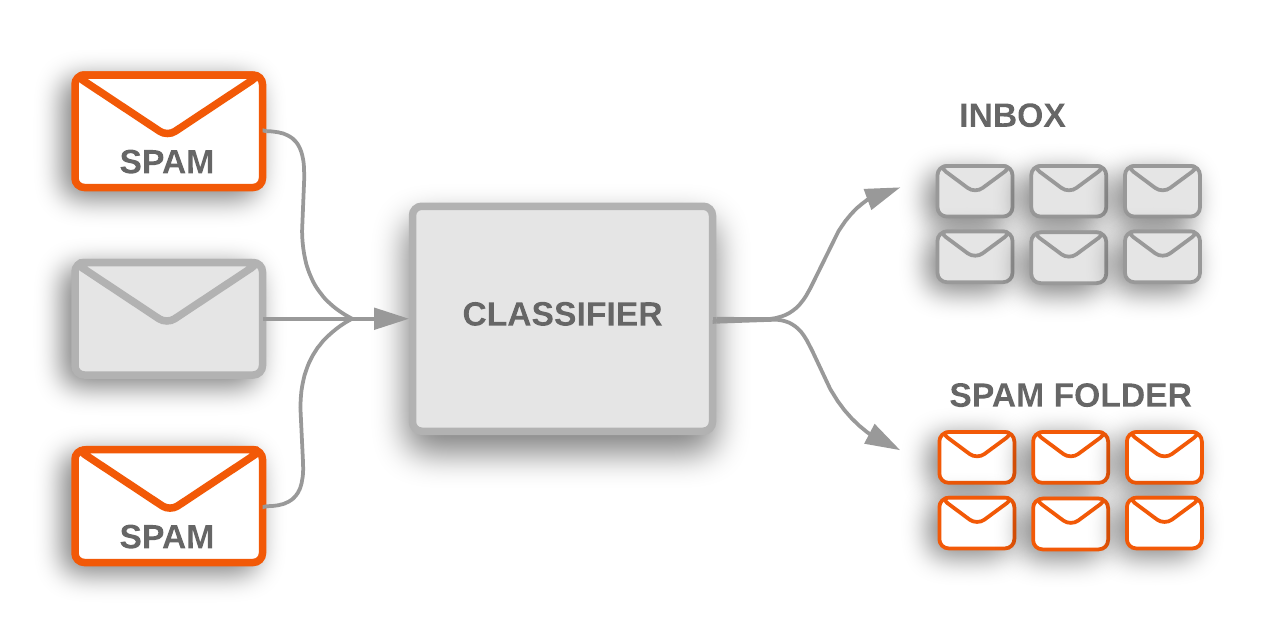
\includegraphics[width=\textwidth]{figures/tc.png}
 \newline
\tiny source: \url{https://developers.google.com/machine-learning/guides/text-classification}
\end{frame}

\begin{frame}
\frametitle{Search}
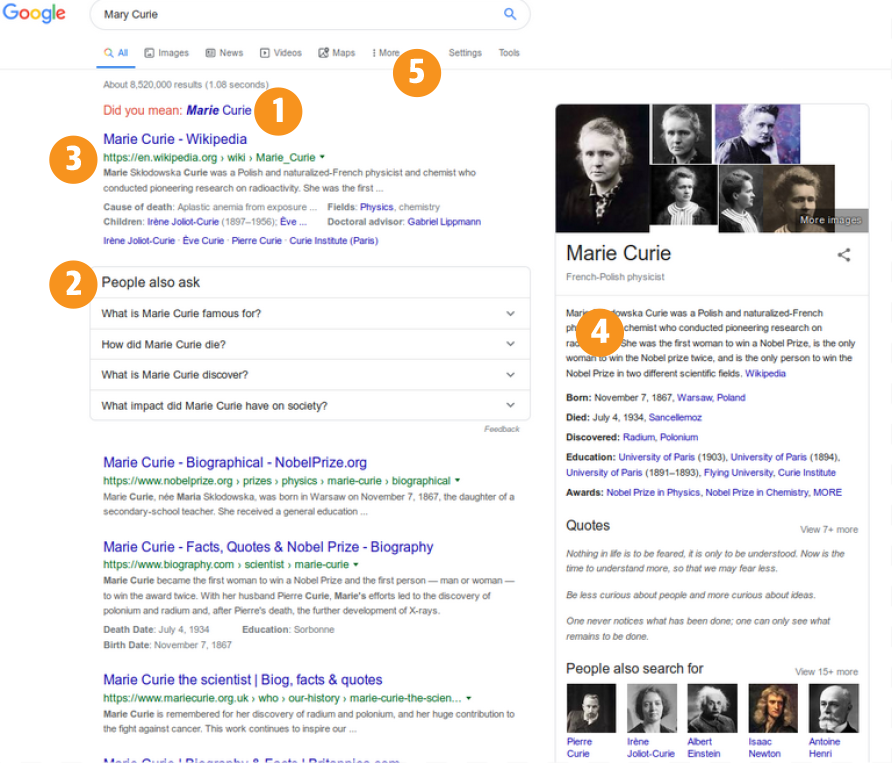
\includegraphics[width=0.8\textwidth]{figures/nlpsearch.png}
\end{frame}

\begin{frame}
\frametitle{Question Answering}
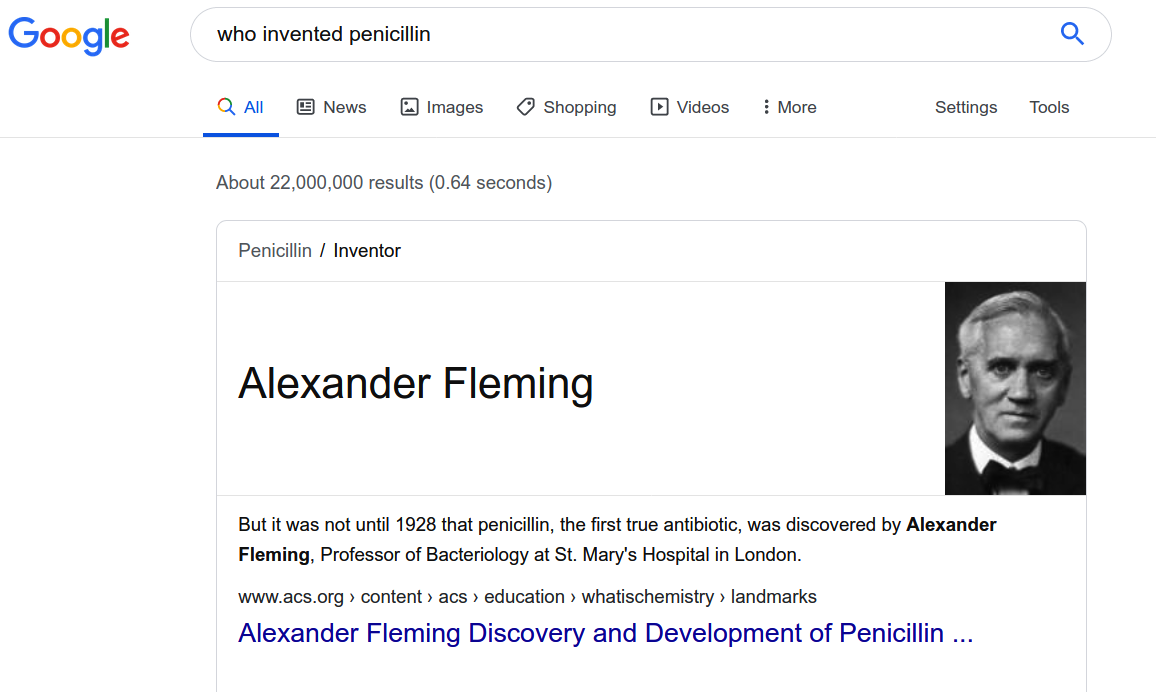
\includegraphics[width=\textwidth]{figures/qa.png}
\end{frame}

\begin{frame}
\frametitle{Information Extraction}
\begin{columns}
    \begin{column}{0.48\textwidth}
 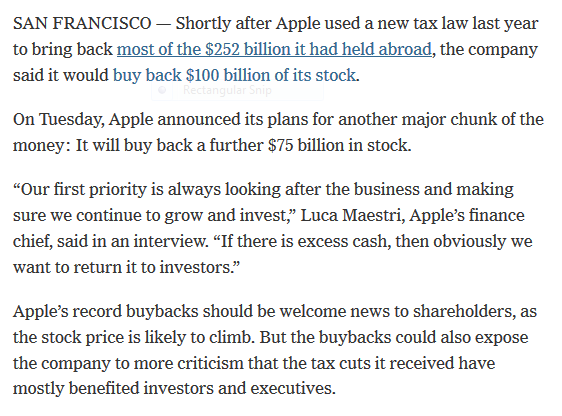
\includegraphics[width=\textwidth>]{figures/ie1.png}
    \end{column}

    \begin{column}{0.48\textwidth}
\begin{itemize} 
\item Who is Luca Mestri?  
  \pause needs: Named Entity Recognition and Linking, Relation extraction
\item What is the article about?  
   \pause needs: Key phrase extraction, event extraction
\end{itemize}
    \end{column}
\end{columns}
\end{frame}

\begin{frame}
\frametitle{Named Entity Extraction/Linking}
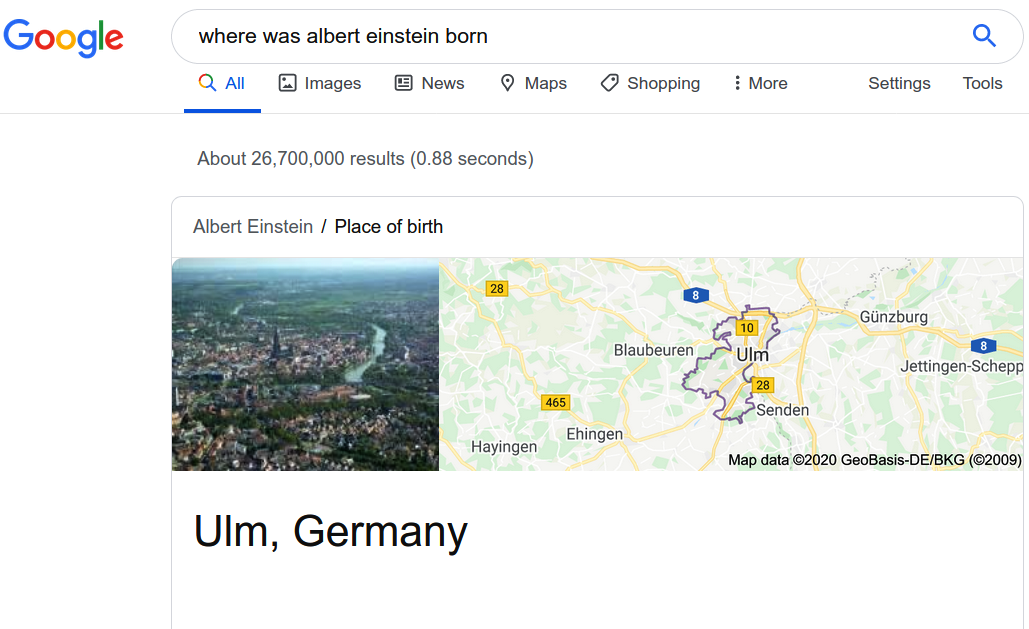
\includegraphics[width=\textwidth]{figures/searchie.png}
\end{frame}


\begin{frame}
\frametitle{Key Phrase Extraction}
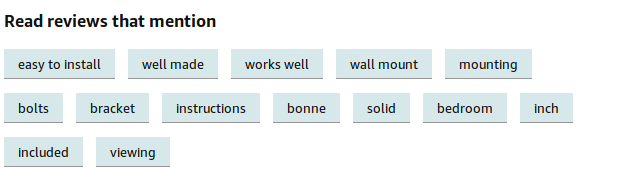
\includegraphics[width=\textwidth]{figures/kpe.png}
\end{frame}

\begin{frame}
\frametitle{Event/Relation Extraction}
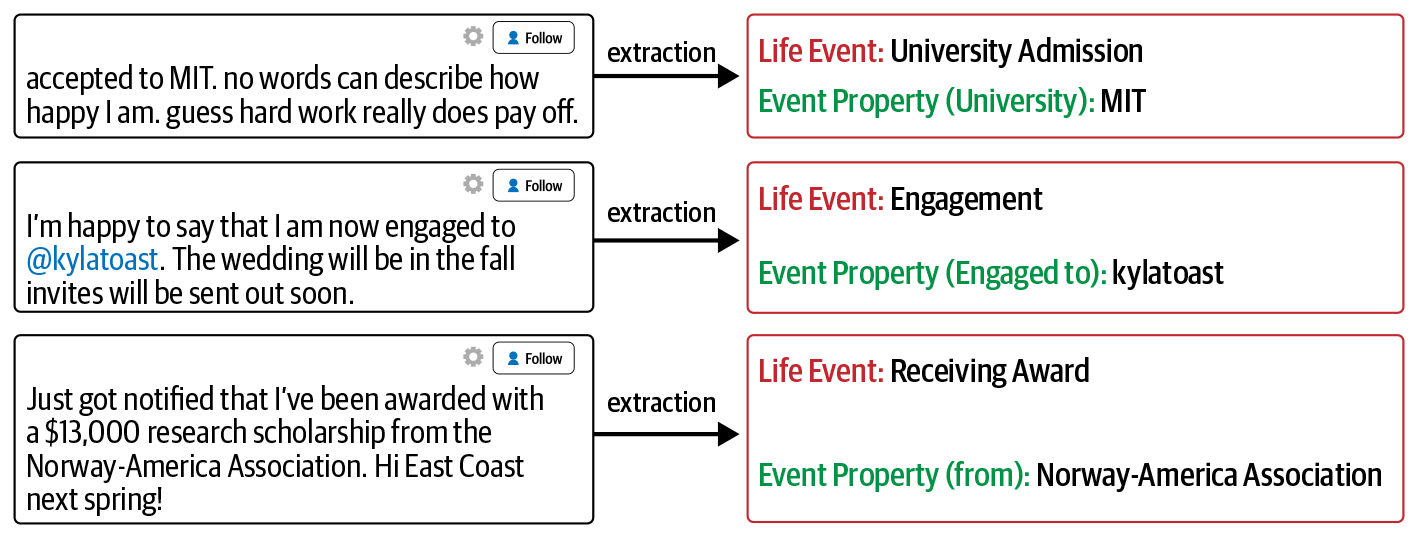
\includegraphics[width=\textwidth]{figures/eventextraction.png}
\end{frame}

\begin{frame}
\frametitle{Chatbots}
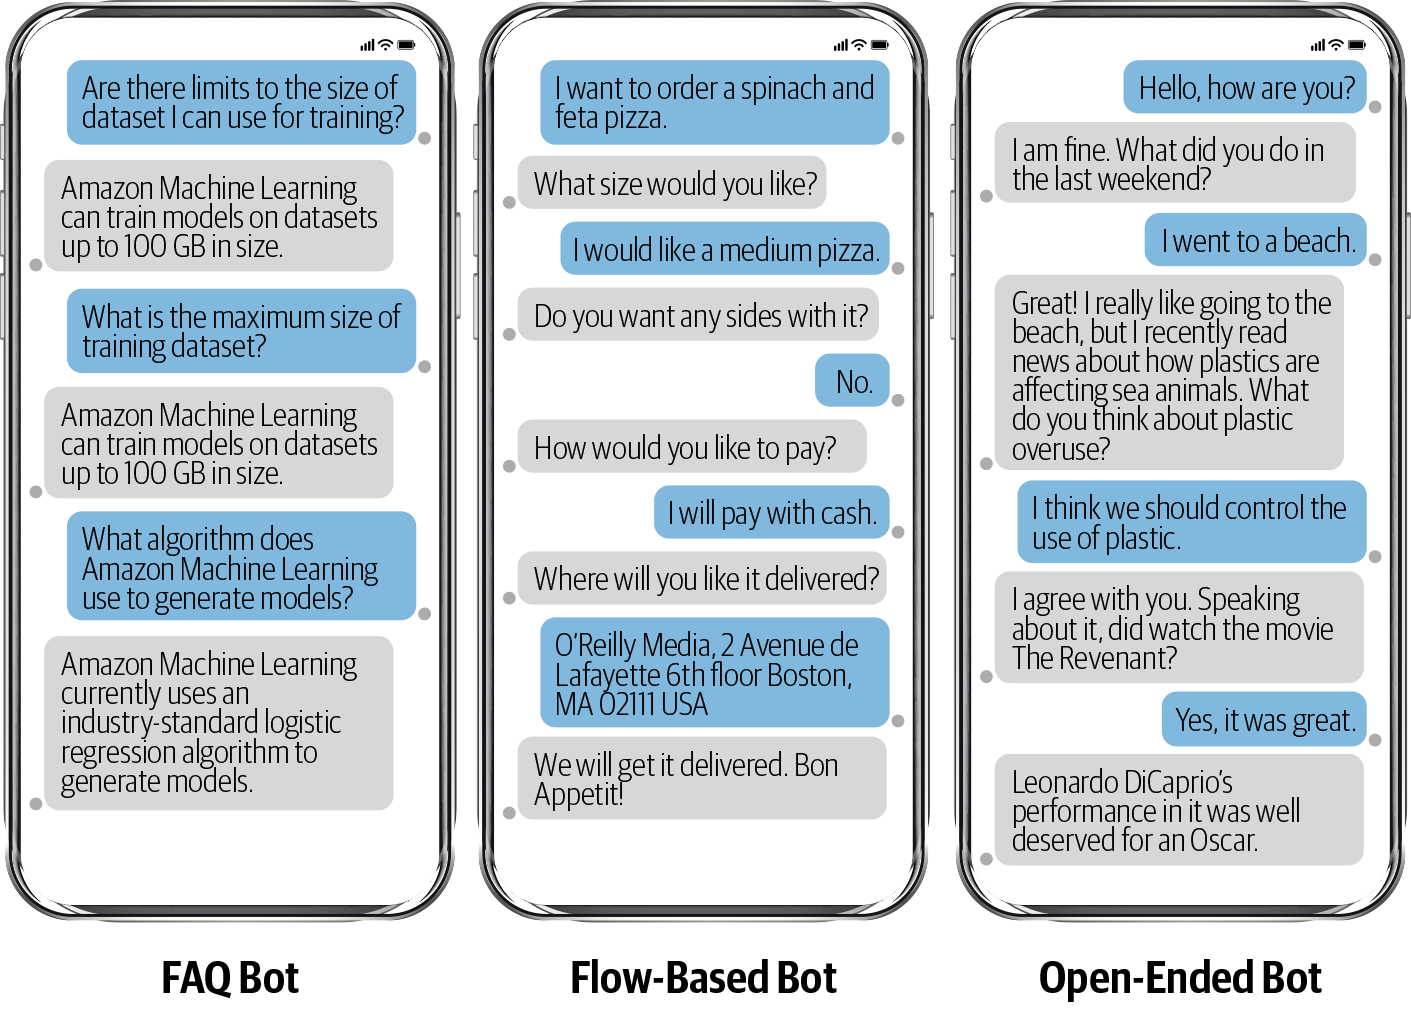
\includegraphics[width=\textwidth]{figures/chatbots.png}
\end{frame}

\begin{frame}
\frametitle{Many more}
\begin{itemize}
\item text summarization
\item text recommendation
\item topic modeling
\item text to speech/speech to text conversion
\item language generation (e.g., automatically generating weather reports, chatbots, etc.)
\end{itemize}
.... and so on.
\end{frame}

\begin{frame}
\frametitle{Outline}
\begin{enumerate}
    \item What is NLP?
    \item The many faces of NLP
    \item What makes NLP Challenging?
    \item Some common NLP Tasks: An overview
    \item \textbf{The levels of language processing: some examples}
    \item Approaches to NLP
\end{enumerate}
\end{frame}

\begin{frame}
\frametitle{Levels of Language Processing}
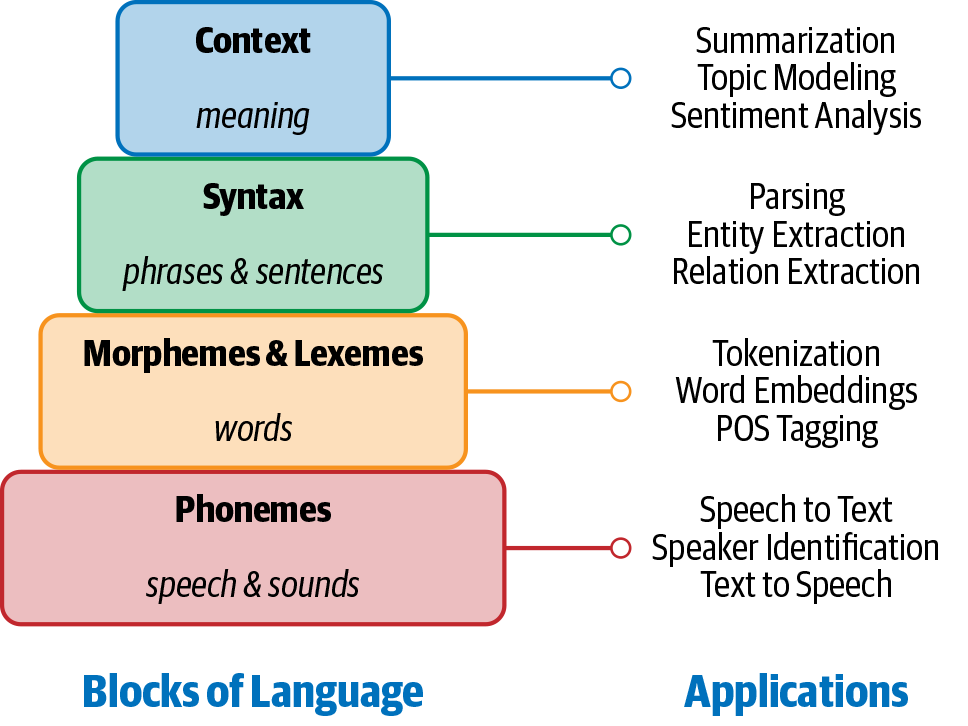
\includegraphics[width=\textwidth]{figures/langblocks.png}
\end{frame}

\begin{frame}
\frametitle{Levels of processing: speech/sounds}
\begin{itemize}
\item What are the sounds of a language? How do they become words? How do we identify them automatically? 
\item Uses: Text to speech conversion, Speech to text conversion, pronunciation training etc
\item Traditionally studied separately under Speech processing. Not a part of NLP courses generally.
\end{itemize}
\end{frame}

\begin{frame}
\frametitle{Levels of processing: Word}
\begin{itemize}
\item Morphological analysis of words
\item compiling lists of words, or word sequences occurring in documents.
\item Understanding/Modeling relationships between words etc. 
\end{itemize}
\end{frame}

\begin{frame}
\frametitle{Levels of processing: Sentence}
\framesubtitle{POS Tagging}
\begin{itemize}
\item Task: Given a sequence of words, return the POS tags for each word.
\item An example problem: What is the best tag for a word in a context?
\begin{itemize}
\item I wish to cite this work. 
\\ PRP/I  VBP/wish  TO/to  VB/cite  DT/this  NN/work ./.
\item He has a wish.
\\ PRP/He  VBZ/has  DT/a  NN/wish ./. 
\end{itemize}
\item Largely considered solved for English, but there are still issues if we go beyond typical newspaper language (e.g., tagging speech or tweets). Still an unsolved problem for several languages.
\end{itemize}
\end{frame}

\begin{frame}
\frametitle{Levels of processing: Sentence}
\framesubtitle{Parsing}
\begin{itemize}
\item Task: Construct the syntactic structure of a given sentence.
\item Two kinds of trees can be generated in NLP: Phrase structure tree (Constituency tree), Dependency tree
\item PST: shows parse structure in terms of Noun Phrases, Verb Phrases, Prep. Phrases etc.
\item Dependency Tree: shows relations between words in a sentence in terms of a pre-defined set of relations
\item Very active area of current research, for multiple languages.
\item Important note: POS tagging errors can carry over and affect parser efficiency. 
\end{itemize}
\end{frame}


\begin{frame}
\frametitle{Levels of processing: Sentence}
\framesubtitle{Word sense disambiguation}
\begin{itemize}
\item Task: For words that can have multiple meanings, what is the right sense of the word in a given sentence? 
\item Example: "Let us go inside, it is cold" vs "I have cold and cough"
\item Very important for applications such as machine translation, information retrieval
\item Good progress for English WSD. One of the active areas of research in the field.
\end{itemize}
\end{frame}

\begin{frame}
\frametitle{Levels of processing: Sentence}
\framesubtitle{Semantic Role Labeling}
\begin{itemize}
\item SRL is all about doing a "semantic parse" of a sentence. The task here is to identify argument structure of a sentence and thematic roles of different entities.
\item Example: (source: \url{http://www.cs.upc.edu/~srlconll/})
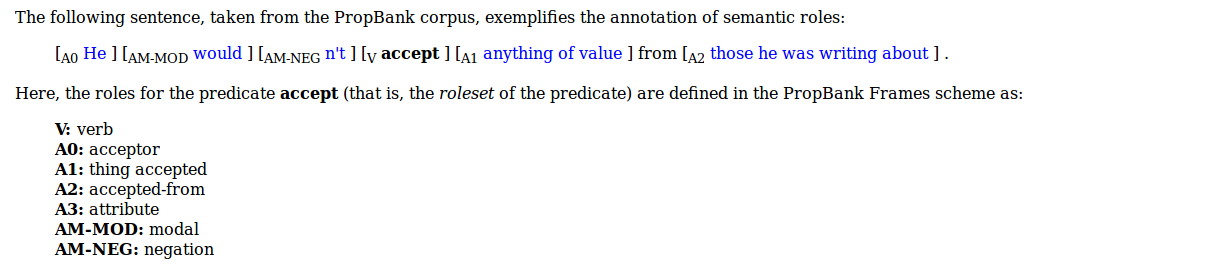
\includegraphics[width=\textwidth]{figures/SRL.png}
\item Active area of research. Still hard, but making progress.
\end{itemize}
\end{frame}


\begin{frame}
\frametitle{Beyond a sentence}
\begin{itemize}
\item Given a text (more than one sentence), analyze the relationships between sentences, identify what pronouns refer to what nouns, how is the same entity referred in different ways (Barack Obama, Obama, The President and so on).
\item What NLP methods are useful: coreference resolution, discourse parsing etc. 
\item Application: Text summarization, Question-Answering, Essay scoring etc.
\item Hard problems, but active research topic and hence, making good progress
\end{itemize}
\end{frame}

\begin{frame}
\Large Questions so far?
\end{frame}

\begin{frame}
\frametitle{Outline}
\begin{enumerate}
    \item What is NLP?
    \item The many faces of NLP
    \item What makes NLP Challenging?
    \item Some common NLP Tasks: An overview
    \item The levels of language processing: some examples
    \item \textbf{Approaches to NLP}
    \item Conclusion
\end{enumerate}
\end{frame}

\begin{frame}{Approaches to NLP}
\begin{enumerate}
    \item heuristics based NLP
    \item machine learning 
    \item deep learning 
    \item combination of all or some of the above three
\end{enumerate}
(More on this in the next class)
\end{frame}

\begin{frame}
\frametitle{Heuristics}
\begin{enumerate}
    \item Word lists, lexicons etc.
    \item Rule engineering based on observed patterns of language use. 
    \item Regular expressions
\end{enumerate}
...
\end{frame}

\begin{frame}
\frametitle{Machine Learning}
\begin{itemize}
    \item Machine learning is a collection of methods that learn a task automatically by looking at lots (and lots) of examples
    \item Usually involves a feature extraction step, where we need to specify what kind of patterns (e.g., words? heuristics? pos tags?) should a machine learn.
    \item Different kinds of machine learning algorithms are used in NLP - naive bayes, logistic regression (text classification), conditional random fields (sequence tagging), clustering etc. 
    \item We will briefly see how some of them are useful for NLP as we progress with the course. 
\end{itemize}
\end{frame}

\begin{frame}
\frametitle{Deep Learning}
\framesubtitle{...a sub-field of machine learning}
\begin{itemize}
    \item  Deep learning is inspired by learning in humans and other biological forms, but "deep" refers to the number of layers in the artificial neural network of the deep learning method. \pause
    \item Some popular deep learning architectures used in NLP in the past 5 years:
    \begin{itemize}
        \item Convolutional Neural Networks are typically used in image processing related problems, and are useful to automatically extract features (words/word sequences) in NLP tasks. 
        \item Transformers (e.g., BERT) model the textual context, but not sequentially. It uses a phenomenon called \textbf{attention} to model the context. 
    \end{itemize} \pause
   Note: Transformers have become very popular in NLP in recent 2-3 years across tasks and languages. 
\end{itemize}
\end{frame}

\begin{frame}
\frametitle{Deep Learning and Transfer Learning}
\begin{itemize}
    \item Deep learning and Machine learning methods in general expect you have to have a lot of data for the problem you want to solve.
    \item Sometimes, we may have a lot of data on some related problem, but very small amount of data on a particular problem.
    \item Transfer learning is all about how to use existing data/knowledge for a new problem. 
\end{itemize}
Transfer learning has also become a popular method in NLP in the recent 2-3 years. 
\end{frame}

\begin{frame}
\Large Questions so far?
\end{frame}

\begin{frame}
\frametitle{Outline}
\begin{enumerate}
    \item What is NLP?
    \item The many faces of NLP
    \item What makes NLP Challenging?
    \item Some common NLP Tasks: An overview
    \item The levels of language processing: some examples
    \item Approaches to NLP
    \item \textbf{Conclusion}
\end{enumerate}
\end{frame}

\begin{frame}
\frametitle{A real world example: revisiting search}
What levels of language processing are involved? What NLP tasks can be seen here? 
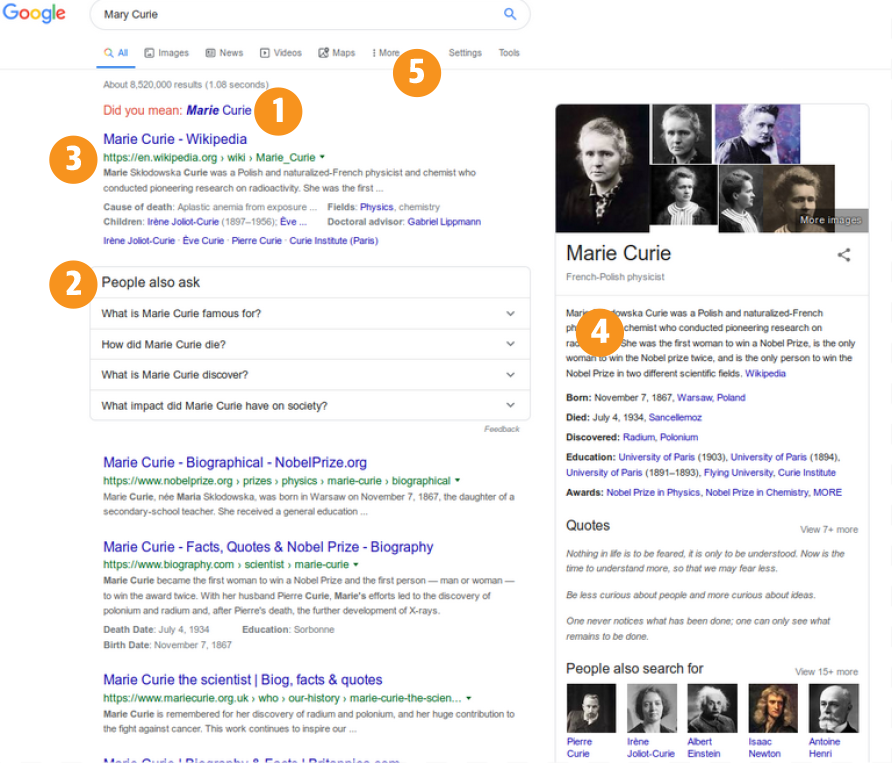
\includegraphics[width=\textwidth]{figures/nlpsearch.png}
\end{frame}
    
\begin{frame}
\frametitle{So, how does one build NLP systems?}
\framesubtitle{NLP Pipeline}
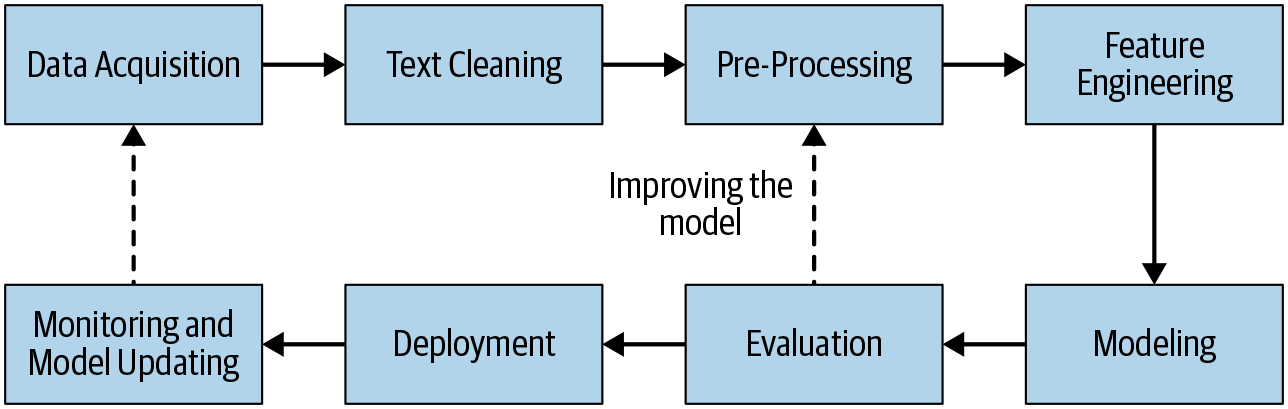
\includegraphics[width=\textwidth]{figures/pipeline.png}
(More on this in the next class!)
\end{frame}

\begin{frame}
\frametitle{ToDo before next meeting} 
\begin{itemize}
\item Take a look at the syllabus document, understand the course requirements, deadlines etc.
\item Read the introductory chapter of any of the textbooks mentioned above for NLP 
\item Check out the assignment descriptions 
\item Decide on a programming language you want to use and setup your laptops for that (e.g., installing any software needed etc)
\item Read Chapter 2 of Practical NLP if you have access. 
\item Please introduce yourselves in the Forum called "Introductions"
\item Ask any questions you have about today in the forum "NLP/Course Overview"
\end{itemize}
\end{frame}

\begin{frame}
\Large Questions so far?
\end{frame}
\end{document}
